\documentclass[25pt,halfparskip-,pagesize]{scrartcl}
\usepackage[papersize={34in,44in},body={780mm,1000mm},top=.5in,ignoreheadfoot]{geometry}
\usepackage{eso-pic}
%\usepackage{bera}
%\usepackage{fourier}
%\usepackage[scaled]{luximono}
\usepackage[T1]{fontenc}
\usepackage[english]{babel}
\usepackage{graphicx,color,multicol,booktabs,listings,fancybox,calc}
\usepackage{capt-of}
\usepackage{subfigure}
%\raggedcolumns
\flushcolumns

%\show\hrulefill
\AddToShipoutPicture{%
    \AtPageUpperLeft{\makebox(0,0)[lt]{\includegraphics[width=\paperwidth]{head-small}}}
    \unitlength1cm
    \AtPageUpperLeft{\kern5cm\lower9cm\hbox{\includegraphics[width=11cm]{../images/GSI_Logo_cmyk.eps}}}
    \AtPageUpperLeft{\kern.1cm\rule[-.3cm]{.4pt}{.2cm}}
    \AtPageUpperLeft{\kern.1cm\rule[-.1cm]{.2cm}{.4pt}}
    \AtPageUpperLeft{\kern\paperwidth\kern-.1cm\rule[-.3cm]{.4pt}{.2cm}}
    \AtPageUpperLeft{\kern\paperwidth\kern-.3cm\rule[-.1cm]{.2cm}{.4pt}}
    \AtPageLowerLeft{\kern.1cm\rule[.1cm]{.4pt}{.2cm}}
    \AtPageLowerLeft{\kern.1cm\rule[.1cm]{.2cm}{.4pt}}
    \AtPageLowerLeft{\kern\paperwidth\kern-.1cm\rule[.1cm]{.4pt}{.2cm}}
    \AtPageLowerLeft{\kern\paperwidth\kern-.3cm\rule[.1cm]{.2cm}{.4pt}}
    \linewidth2pt
    \AtPageLowerLeft{\kern1in\kern\oddsidemargin\lower-3cm\hbox to \textwidth{\leaders \hrule height \linewidth \hfill \kern 1cm\lower.5cm\hbox{\includegraphics[height=2cm]{../images/GSI_Logo_cmyk.eps}}\kern1cm\rule{3cm}{\linewidth}}}
    \AtPageLowerLeft{\kern1in\kern\oddsidemargin\lower-2cm\hbox{\sffamily\fontsize{12pt}{12pt}\selectfont ICALEPCS\,2011}}
}

\def\TTra{\textsuperscript{\texttrademark}}
\definecolor{title}{cmyk}{.00,0.15,0.75,0}
\definecolor{solution}{cmyk}{.10,1.00,.80,0}
%\definecolor{colsection}{cmyk}{1,.8,0,0}
\definecolor{colsection}{cmyk}{0,.6,.6,.7}
\definecolor{itemgreen}{cmyk}{1,0,.9,.2}
\definecolor{itemroyalblue}{cmyk}{.711,.533,0,.118}
\definecolor{itemblue}{cmyk}{1,1,0,.2}
\definecolor{lstbackground}{cmyk}{0.35,0.05,0.0,0.0}
\definecolor{lstemph}{cmyk}{0.0,1.0,0.95,0.0}
\definecolor{lstbackgroundalt}{cmyk}{0.05,0.05,0,0.2}
\definecolor{lststring}{cmyk}{.6,1,.8,0}
\newcommand{\solution}[1]{\textbf{\textcolor{solution}{#1}}}
\setkomafont{descriptionlabel}{\itshape}
\setcounter{secnumdepth}{-1}
\pagestyle{empty}
\addtokomafont{section}{\color{colsection}}
\addtokomafont{caption}{\itshape}
\setlength{\columnsep}{5em}
\newcommand\mycaption[1]{\textit{#1}}
%\renewcommand{\familydefault}{\rmdefault}

\usepackage{pifont}
\renewcommand*\labelitemi{\color{colsection}\ding{110}}
\renewcommand*\labelitemii{\color{itemgreen}\ding{108}}

\lstset{showstringspaces=false,basicstyle=\ttfamily\small,
    keywordstyle={\bfseries},stringstyle={\color{lststring}},tabsize=4,framerule=2pt,rulecolor=\color{black},
    rulesep=5pt,abovecaptionskip=6pt,belowcaptionskip=8pt,
    emphstyle=\color{lstemph}}

\lstdefinelanguage{nodal}
}

\newcommand\class[1]{\texttt{#1}}

\makeatletter
\DeclareRobustCommand{\Cpp}
{\valign{\vfil\hbox{##}\vfil\cr
   C\kern-.05em\cr
      %$\hbox{\fontsize{\sf@size}{0}+\kern-0.05em+}$\cr}%
      \hbox{+\kern-0.05em+}\cr}%
}
\makeatother

\setlength{\fboxsep}{1em}
\raggedright
\begin{document}
\vspace*{1ex}

{\centering
\begin{minipage}{20in}
\centering \sffamily\Huge \rule{0pt}{50pt}\textbf{PERFORMANCE OF THE STANDARD FAIR EQUIPMENT CONTROLLER PROTOTYPE}\par
\vspace{5mm} \LARGE Stefan Rauch, Ralph C. B\"ar, Wolfgang Panschow, Matthias Thieme
\par
\vspace{5mm}
\Large\itshape GSI, Darmstadt, Germany
\rule[-12pt]{0pt}{10pt}\par
\end{minipage}%
\par}%

\vspace{11cm}
\setlength{\fboxrule}{1pt}
\begin{multicols*}{3}
\ovalbox{%
\begin{minipage}{\linewidth}
\section{Abstract}
\small For the control system of the new FAIR accelerator facility a standard equipment controller, the Scalable Control Unit (SCU), is presently under development. First prototypes have already been tested in real applications. The controller combines an x86 COM Express\TTra Board and an Altera Arria\TTra II FPGA. Over a parallel bus interface called the SCU bus, up to 12 slave boards can be controlled. Communication between CPU and FPGA is done by a PCIe link. We discuss the real time behaviour between the Linux OS and the FPGA Hardware. For the test, a Front-End Software Architecture (FESA) class, running under Linux, communicates with the PCIe bridge in the FPGA. Although we are using PCIe only for single 32 bit wide accesses to the FPGA address space, the performance still is sufficient. The tests showed an average response time to IRQs of 50 $\mu s$ with a 1.6 GHz Intel Atom CPU. This includes the context change to the FESA user space application and the reply back to the FPGA. Further topics are the bandwidth of the PCIe link for single/burst transfers and the performance of the SCU bus communication.
\par
\end{minipage}}



%\par
%\vfill

\section{Description of the SCU}
\begin{itemize}
	\item SCUB connections with LVDS and PCIe
	\begin{itemize}
		\item strict Master/Slave bus
		\item 16Bit data bus, 16Bit address bus
		\item in addition serial LVDS and PCIe channels
	\end{itemize}
	\item COM Express\TTra module Type II with Intel Atom
	\item 32Mbyte Parallel Flash
	\item RJ45 Gigabit Ethernet from COM Express\TTra module
	\item two SFP connectors
	\begin{itemize}
		\item Timing (White Rabbit over GbE)
		\item AUX LAN (GbE)
	\end{itemize}
	\item Arria\TTra II FPGA
	\item White Rabbit Timing Receiver (FPGA)
	\item 128Mbyte DDR3 memory
%	\columnbreak
	\item IO Extension for existing timing system
	\begin{itemize}
		\item DEV-BUS: GSI fieldbus
		\item Event-In: Timing Events
		\item both based on MIL-STD-1553
	\end{itemize}
	\item USB 2.0
	\item 2x EIA-232
\end{itemize}



\includegraphics[angle={90}, width=\columnwidth]{../images/WEPMN018f2}
\captionof{figure}{Carrier Board Layout}

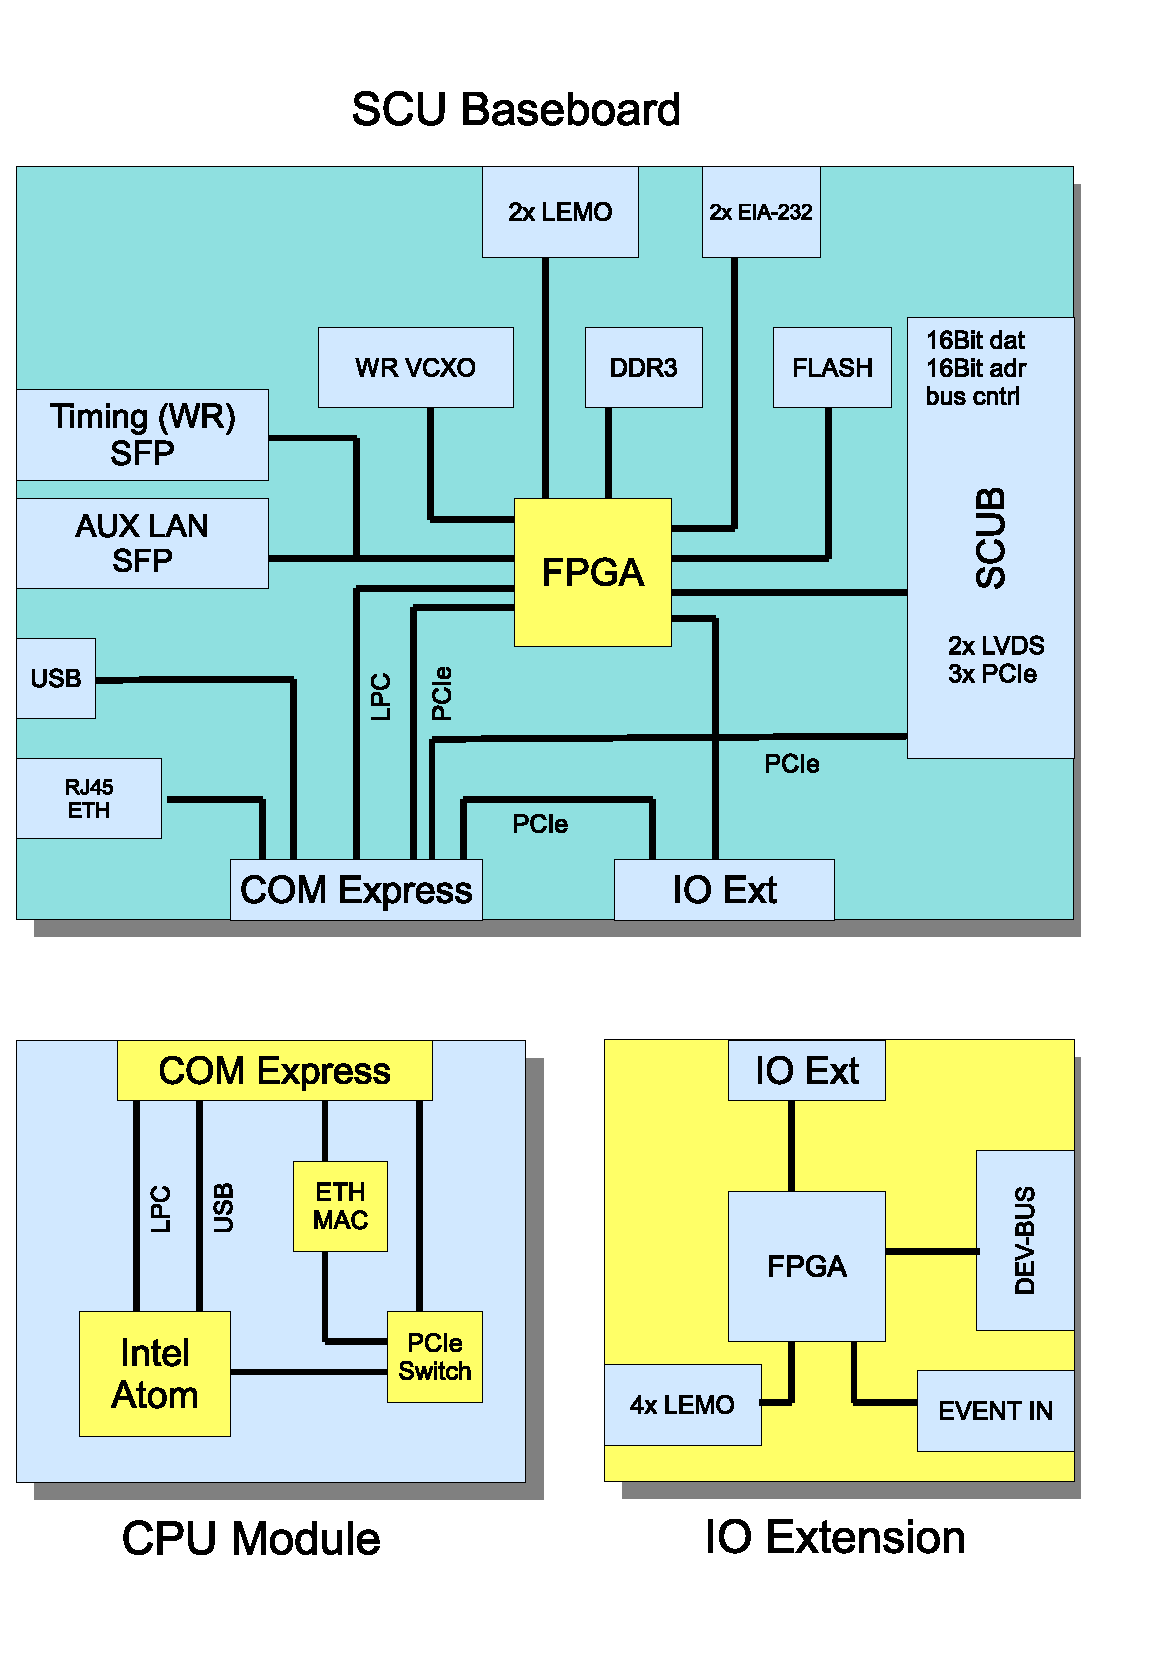
\includegraphics[width=\columnwidth]{../images/scu_schema}
\captionof{figure}{SCU schematic}




%\begin{figure}
%\subfigure[Bildunterschrift]{\includegraphics[width=0.49\columnwidth]{../images/WEPMN018f2}}\hfill
%\subfigure[Bildunterschrift]{\includegraphics[width=0.49\columnwidth]{../images/WEPMN018f3}}
%\caption{Gesamtbild-Unterschrift}
%\end{figure}

%\begin{minipage}[hbt]{0.5\columnwidth}
%	\centering
%	\includegraphics[width=0.49\columnwidth]{../images/WEPMN018f2}
%	\caption{Carrier Board Layout}
%	\label{Bild2}
%\end{minipage}
%\hfill
%\begin{minipage}[hbt]{0.49\columnwidth}
%	\centering
%	\includegraphics[width=0.49\columnwidth]{../images/WEPMN018f3}
%	\caption{Front Panel}
%	\label{Bild3}
%\end{minipage}

%\includegraphics[width=0.49\columnwidth]{../images/WEPMN018f2}
%\captionof{figure}{Layout of the SCU Carrier Board}


\includegraphics[width=0.6\columnwidth]{../images/WEPMN018f3}
\captionof{figure}{Front Panel}


\par

\section{Problems during design phase}
\begin{itemize}
	\item fitting of high speed serial transceivers
	\item timing issues with DDR3 memory controller
	\item errors with DDR3 communication
	\item layout errors based on unclear documentation and design tool errors
\end{itemize}
The Arria\TTra FPGA comes with a hard IP cell for PCIe so no license fees are needed. This FPGA and the design tools were quite new, when the testing of base components of the system like PCIe or DDR3 communication began. In FPGA prototyping you typically implement the design first in the FPGA due to constraints in the pinning of the PCB. In this special case, the design tool allowed the hard IP cell to be connected to the transceiver block 1 of the Arria\TTra. The problem is, there is no hardware connection in the FPGA and the PCBs did not run PCIe with the hard IP cell. One possibility to solve this problem was the use of a soft core implementation. This would result in high license fees and unnecessary loss of logic cells in the FPGA. Another temporary solution was rewiring the PCB. After patching the PCIe to transceiver block 0 the connection worked perfectly. Altera fixed the issue in the next version of their design tool, but for the final solution a redesign of the PCB was needed.

\section{Lessons Learned}
\begin{itemize}
	\item plan a lot more time for testing new technologies
	\item new FPGAs with high speed transceivers and mem controllers have lots of constraints
	\item a lot of independent clock inputs are needed for optimal routing
	\item layout errors based on unclear documentation and design tool errors
	\item the HDL design has to be frozen early in the project
	\item most changes cannot be made after PCB is finished
\end{itemize}


\section{In Detail: Implementing a LPC UART}
\begin{itemize}
	\item Problem: SuperIO Chip does not fit in Layout
	\item Solution: extending LPC bus to FPGA, implementing UART functionality in logic
	\item Low Pin Count Bus, four address/data lines, serial clk, frame signal
	\item running at 33MHz
	\item IO read/write, MEM read/write
	\item 16750 compatible UART core
	\item Whishbone LPC Peripheral Bridge
	\item emulating extended function mode of SuperIO chip
	\item up to 11 devices, e.g. UARTs, printer port, MIDI
	\item base address of UART can be configured
	\item 16750 UART is then mapped to 
\end{itemize}

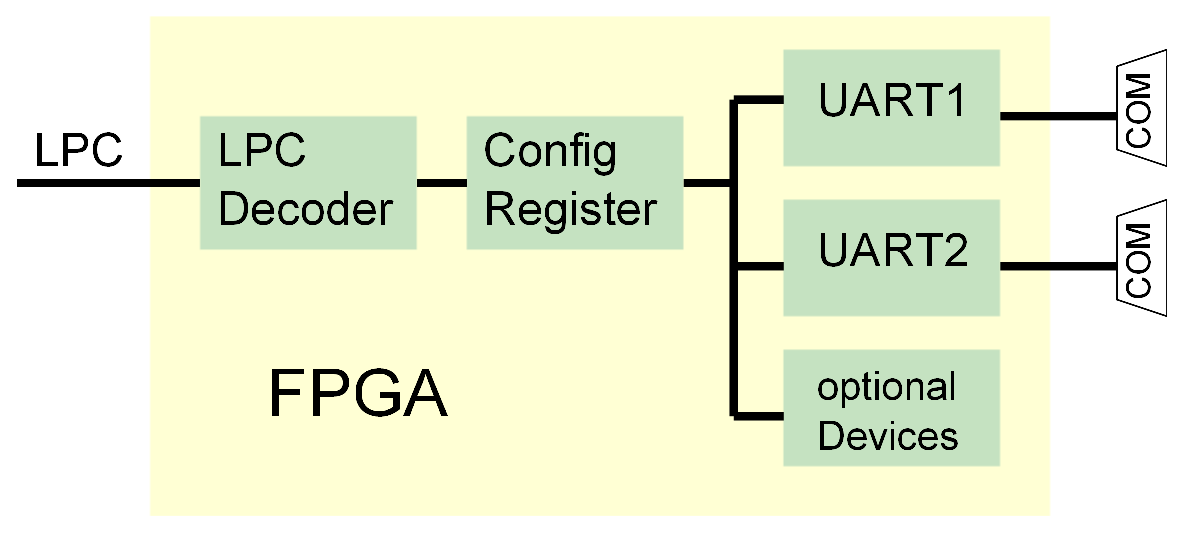
\includegraphics[width=\columnwidth]{../images/lpc_schema.eps}
\captionof{figure}{LPC UART schematic}

\section{Status Report of the Project}
The prototype should have been ready in July 2011, but to complications during the design phase it came to a delay. The layout for the prototype baseboard is now finished and ready for production. The first boards are expected to be shipped in November 2011. 

%\section{``''}
%\begin{itemize}
%\item[\color{itemroyalblue}\ding{55}]
%\item[\color{itemroyalblue}\ding{55}]
%\item[\color{itemroyalblue}\ding{55}]
%\end{itemize}
\vfill

\end{multicols*}
\end{document}
